% ============================================================
%  CHAPTER 4: SYSTEM ARCHITECTURE AND DESIGN
% ============================================================

\chapter{SYSTEM ARCHITECTURE AND DESIGN}
\label{chap:system_design}

\section{Overall Architecture and Network Topology}
\label{sec:overall_architecture}

QuantumSafe VPN implements an end-to-end, post-quantum secure tunneling architecture between an unprivileged Android client and a hardened Linux security gateway. As illustrated in Figure~\ref{fig:deployment_topology}, the system partitions responsibilities across three discrete layers:
\begin{enumerate}
    \item Android Client Layer: Captures user-space IP traffic through the \texttt{android.net.}\allowbreak\texttt{VpnService} API, negotiates ephemeral lattice keys via pure-Kotlin PQC primitives, and encapsulates raw datagrams inside authenticated frames.
    \item Untrusted WAN Transit Layer: Transports length-prefixed, ciphertext frames over TCP port 7000.
    \item Linux Gateway Layer: Authenticates incoming sessions via ML-DSA-65 signatures, decapsulates ML-KEM-1024 shared secrets, leases private virtual IPv4 addresses, and performs kernel-level IP forwarding and Network Address Translation (NAT).
\end{enumerate}

\begin{figure}[!t]
  \centering
  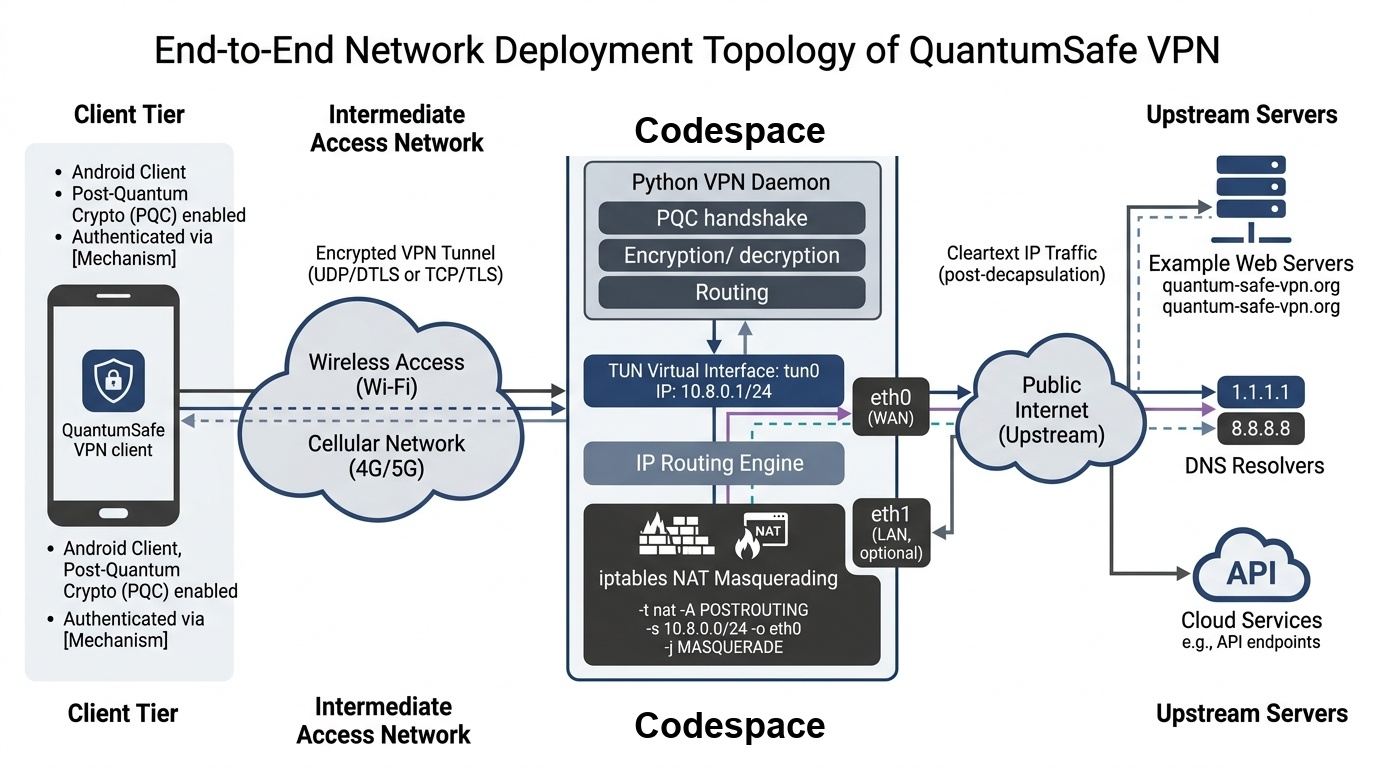
\includegraphics[width=0.88\linewidth,height=0.30\textheight,keepaspectratio]{figures/deployment_topology_concept.jpg}
  \caption[End-to-End Network Deployment Topology]{End-to-End Network Deployment Topology and Component Placement.}
  \label{fig:deployment_topology}
\end{figure}

\section{Binary Wire Framing Specification}
\label{sec:wire_framing_design}

Every frame transmitted over the TCP stream begins with a mandatory 4-byte big-endian length prefix, followed by the authenticated payload structure illustrated in Figure~\ref{fig:tikz_packet_framing}:
\begin{equation}
\label{eq:wire_framing_equation}
\begin{split}
\text{Wire Frame} = {} & \underbrace{[\text{Length} : 4\text{B}]}_{\text{Framing}} \parallel \underbrace{[IV : 12\text{B}]}_{\text{Nonce}} \parallel \underbrace{[\text{Auth Tag} : 16\text{B}]}_{\text{Galois MAC}} \\
& \parallel \underbrace{\text{AES-GCM}_{\text{Key}}\Big([\text{Seq} : 8\text{B}] \parallel [\text{Raw IPv4 Datagram}]\Big)}_{\text{Encrypted Payload}}
\end{split}
\end{equation}

\begin{figure}[!b]
  \centering
  \begin{tikzpicture}[
    scale=0.80, every node/.style={transform shape},
    field/.style={draw=darkcharcoal, thick, fill=white, minimum height=1.1cm, align=center, font=\footnotesize\bfseries},
    headerfield/.style={field, fill=blue!10},
    ivfield/.style={field, fill=teal!10},
    seqfield/.style={field, fill=yellow!15},
    payloadfield/.style={field, fill=vpnblue!15},
    tagfield/.style={field, fill=red!10}
  ]
    \node[headerfield, minimum width=2.2cm] (len) at (0, 0) {Length\\(4B)};
    \node[ivfield, minimum width=2.4cm] (iv) at (2.3, 0) {GCM Nonce\\(12B)};
    \node[seqfield, minimum width=2.4cm] (seq) at (4.7, 0) {Monotonic Seq\\(8B)};
    \node[payloadfield, minimum width=4.5cm] (data) at (8.2, 0) {Raw IPv4 Datagram\\(Up to MTU)};
    \node[tagfield, minimum width=2.4cm] (tag) at (11.7, 0) {Auth Tag\\(16B)};

    \draw[thick, decorate, decoration={brace, amplitude=5pt, mirror}] (-1.1, -0.8) -- (12.9, -0.8)
      node[midway, yshift=-0.45cm, font=\footnotesize\bfseries] {Total Wire Frame Transmitted over TCP Stream};

    \draw[thick, decorate, decoration={brace, amplitude=5pt}] (3.5, 0.8) -- (10.5, 0.8)
      node[midway, yshift=0.45cm, font=\scriptsize\bfseries, text=vpnblue] {Encrypted \& Authenticated via AES-256-GCM};
  \end{tikzpicture}
  \caption{Binary Wire Framing and Packet Encapsulation Format.}
  \label{fig:tikz_packet_framing}
\end{figure}

\section{Cryptographic Handshake Protocol Sequence}
\label{sec:handshake_sequence}

Figure~\ref{fig:tikz_handshake_seq} details the four-stage post-quantum cryptographic handshake establishing the tunnel session:
\begin{enumerate}
    \item Stage 1 (Server Identity): The gateway transmits its static ML-DSA-65 public key (1,952 bytes).
    \item Stage 2 (Client Ephemeral KEM): The client generates an ephemeral ML-KEM-1024 keypair and dispatches its public key (1,568 bytes).
    \item Stage 3 (Encapsulation and Signature): The gateway encapsulates a 32-byte shared secret, signs the session transcript using ML-DSA-65 (3,309 bytes signature), and appends the JSON network lease configuration.
    \item Stage 4 (Key Derivation): Both endpoints independently derive an identical 256-bit symmetric key via HKDF-SHA256 (RFC 5869) and configure their local TUN routing adapters.
\end{enumerate}

\begin{figure}[!t]
  \centering
  \begin{tikzpicture}[
    scale=0.80, every node/.style={transform shape},
    lifeline/.style={thick, dashed, draw=mutedgrey},
    nodeblock/.style={draw=darkcharcoal, thick, fill=white, rounded corners=3pt, minimum width=2.8cm, minimum height=0.9cm, align=center, font=\footnotesize\bfseries},
    msg/.style={thick, ->, >=stealth, font=\scriptsize}
  ]
    \node[nodeblock] (ui) at (0, 0) {Android UI\\(Compose)};
    \node[nodeblock] (vpn) at (3.5, 0) {VpnService\\(Worker Threads)};
    \node[nodeblock] (pqc) at (7.0, 0) {PQC Engine\\(ML-KEM/DSA)};
    \node[nodeblock] (srv) at (11.0, 0) {VPN Server\\(tunnel\_server.py)};

    \draw[lifeline] (ui) -- ++(0, -8.5);
    \draw[lifeline] (vpn) -- ++(0, -8.5);
    \draw[lifeline] (pqc) -- ++(0, -8.5);
    \draw[lifeline] (srv) -- ++(0, -8.5);

    \draw[msg] (0, -0.8) -- node[above] {User taps Connect} (3.5, -0.8);
    \draw[msg] (3.5, -1.4) -- node[above] {protect(socket)} (3.5, -1.8);
    \draw[msg] (3.5, -2.3) -- node[above] {TCP Connect (Port 7000)} (11.0, -2.3);

    \draw[msg] (11.0, -3.0) -- node[above] {Stage 1: Server ML-DSA-65 PK (1952B)} (3.5, -3.0);
    \draw[msg] (3.5, -3.5) -- node[above] {Generate Ephemeral ML-KEM} (7.0, -3.5);
    \draw[msg] (7.0, -4.2) -- node[above] {Stage 2: Client ML-KEM-1024 PK (1568B)} (11.0, -4.2);

    \draw[msg] (11.0, -4.9) -- node[above] {Encapsulate \& Sign Transcript} (11.0, -5.3);
    \draw[msg] (11.0, -5.9) -- node[above] {Stage 3: Ciphertext (1568B) + Sig (3309B) + Config} (3.5, -5.9);

    \draw[msg] (3.5, -6.5) -- node[above] {Verify Sig \& Decapsulate Secret} (7.0, -6.5);
    \draw[msg] (7.0, -7.2) -- node[above] {Derive Session Key (HKDF-SHA256)} (7.0, -7.6);
    \draw[msg] (3.5, -8.0) -- node[above] {State: CONNECTED} (0, -8.0);
  \end{tikzpicture}
  \caption[UML Sequence Diagram: 4-Stage Post-Quantum Handshake]{UML Sequence Diagram: 4-Stage Post-Quantum Cryptographic Handshake.}
  \label{fig:tikz_handshake_seq}
\end{figure}

\section{UML Class Hierarchy}
\label{sec:uml_class_hierarchy}

Figure~\ref{fig:tikz_uml_class} depicts the object-oriented structure of the Android client application adhering to the Model-View-ViewModel (MVVM) architectural pattern.

\begin{figure}[!b]
  \centering
  \begin{tikzpicture}[
    scale=0.80, every node/.style={transform shape},
    classbox/.style={draw=darkcharcoal, thick, fill=white, rounded corners=2pt, align=left, font=\scriptsize}
  ]
    \node[classbox, minimum width=5.5cm] (vm) at (0, 3.8) {
      \textbf{\large VpnViewModel}\\
      \rule{5.4cm}{0.4pt}\\
      - \texttt{\_uiState: MutableStateFlow<VpnUiState>}\\
      - \texttt{\_telemetry: MutableStateFlow<TelemetryData>}\\
      \rule{5.4cm}{0.4pt}\\
      + \texttt{connect(host: String, port: Int): Unit}\\
      + \texttt{disconnect(): Unit}
    };

    \node[classbox, minimum width=6.2cm] (vpn) at (0, -0.8) {
      \textbf{\large QuantumSafeVpnService}\\
      \rule{6.1cm}{0.4pt}\\
      - \texttt{vpnInterface: ParcelFileDescriptor?}\\
      - \texttt{socketChannel: SocketChannel?}\\
      - \texttt{pqcEngine: PqcEngine}\\
      \rule{6.1cm}{0.4pt}\\
      + \texttt{onStartCommand(intent: Intent, ...): Int}\\
      + \texttt{connectVpn(host: String, port: Int, ...): Unit}
    };

    \node[classbox, minimum width=5.6cm] (pqc) at (7.2, -0.8) {
      \textbf{\large PqcEngine}\\
      \rule{5.5cm}{0.4pt}\\
      - \texttt{sessionKey: ByteArray?}\\
      \rule{5.5cm}{0.4pt}\\
      + \texttt{generateKemKeyPair(): KemKeyPair}\\
      + \texttt{decapsulateKem(sk: ByteArray, c: ByteArray): ByteArray}\\
      + \texttt{encryptAesGcm(key: ByteArray, p: ByteArray, s: Long): ByteArray}
    };

    \draw[thick, ->] (vm.south) -- node[right, font=\tiny\bfseries] {binds \& controls} (vpn.north);
    \draw[thick, ->] (vpn.east) -- node[above, font=\tiny\bfseries] {delegates crypto} (pqc.west);
  \end{tikzpicture}
  \caption{UML Class Hierarchy of Android Client Architecture.}
  \label{fig:tikz_uml_class}
\end{figure}
